\chapter{Implémentation et réalisation des dashboards Power BI}

\section{Artefact inspecté}
Le dépôt contient Smart\_Industrial\_Maintenance.pbix, ainsi que trois captures correspondant aux pages du rapport. Les captures ont été examinées directement. Le texte ci-dessous décrit les visuels visibles et ne prétend pas décrire des éléments non présents sur les images.

Les trois fichiers disponibles mesurent respectivement 785$\times$482, 791$\times$485 et 793$\times$486 pixels. Les originaux présents dans reports/figures et leurs copies dans le dossier du rapport ont les mêmes dimensions et tailles. Aucune capture HD de 1600 ou 1920 pixels n'a été trouvée ; les images ne sont donc pas artificiellement agrandies. Pour une version de soutenance plus lisible, il faudra reprendre manuellement chaque page dans Power BI Desktop en résolution native élevée ou exporter le rapport, puis remplacer les fichiers sans modifier leurs proportions.

\begin{table}[H]
\centering
\caption{Visuels, champs et filtres vérifiés dans les trois dashboards}
\label{tab:dashboard-fields}
\begin{tabularx}{\textwidth}{>{\bfseries}l X X}
\toprule
Page & Champs ou mesures visibles & Filtres et lecture\\
\midrule
Vue générale & Nombre observations, Nombre incidents documentés, Observations dans incidents documentés, Taux observations incidentées ; date et durée par rapport. & Contexte global ; les creux temporels représentent une couverture variable.\\
Surveillance des capteurs & Date/CalendarDate ; moyenne de TP3, Oil\_temperature et Motor\_current. & Sélection temporelle ; lecture conjointe des signaux sans seuil métier ajouté.\\
Incidents et OLAP & FailureReportCode, FailureType, Severity, DurationSeconds, observations par incident, Year et Hour. & MonthName et Hour ; slice, dice et pivot visibles, drill-down à confirmer selon la hiérarchie active.\\
\bottomrule
\end{tabularx}
\end{table}

\section{Dashboard 1 -- Vue générale}
\begin{figure}[H]
\centering
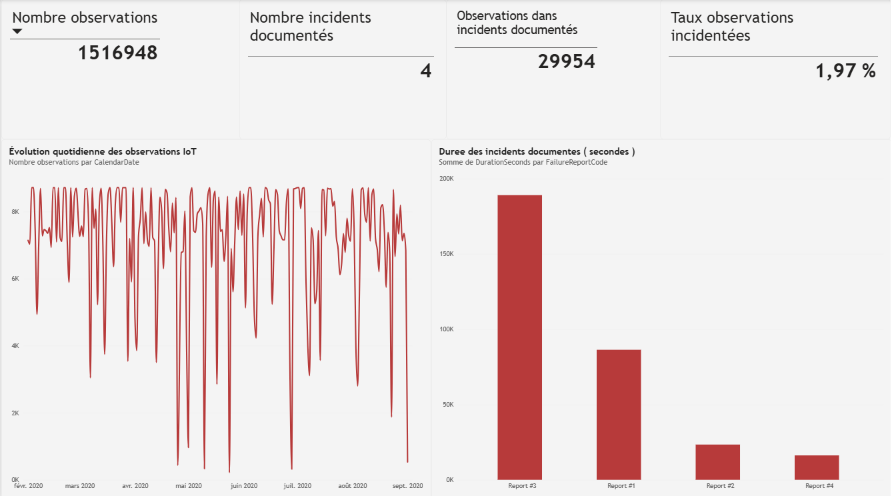
\includegraphics[width=\textwidth]{dashboard_1_vue_generale.png}
\caption{Page Power BI Vue générale}
\label{fig:dashboard1}
\sourcefigure{capture réelle présente dans reports/figures}
\end{figure}
La page comporte quatre cartes. Nombre observations affiche 1\,516\,948. Nombre incidents documentés affiche 4. Observations dans incidents documentés affiche 29\,954. Taux observations incidentées affiche 1,97\,\%. La courbe inférieure montre l'évolution quotidienne du nombre d'observations ; les creux visibles signalent une couverture quotidienne variable, et non nécessairement une panne. L'histogramme présente la durée des incidents documentés en secondes : le rapport 3 est le plus long, suivi des rapports 1, 2 et 4.

\section{Dashboard 2 -- Surveillance des capteurs}
\begin{figure}[H]
\centering
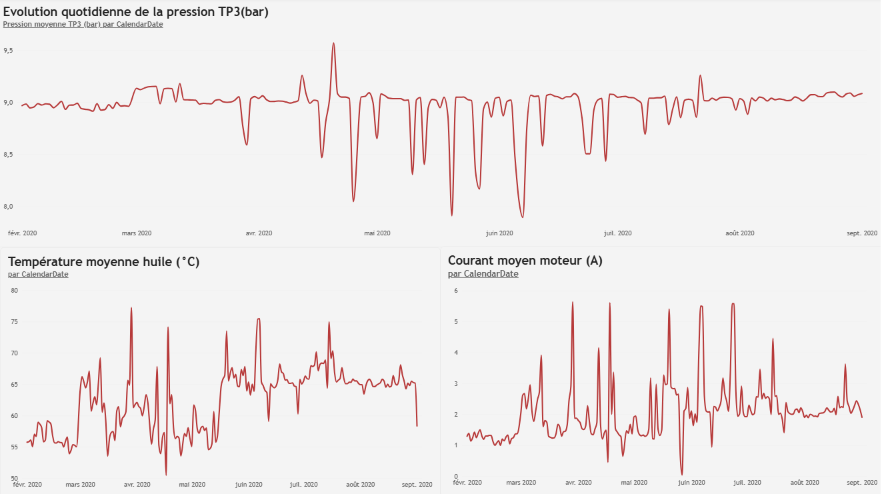
\includegraphics[width=\textwidth]{dashboard_2_surveillance_capteurs.png}
\caption{Page Power BI Surveillance des capteurs}
\label{fig:dashboard2}
\sourcefigure{capture réelle présente dans reports/figures}
\end{figure}
La page montre une courbe de la pression moyenne TP3, une courbe de température moyenne d'huile et une courbe de courant moyen du moteur. TP3 reste proche de 9 bar sur de nombreuses périodes mais présente des baisses ponctuelles jusqu'à environ 7,9 bar dans la visualisation. La température varie approximativement entre 53 et 77 degré C selon les dates affichées. Le courant présente une ligne de base autour de 1 à 3 A avec plusieurs pics visibles jusqu'à environ 5,6 A.

Ces amplitudes sont des lectures visuelles des axes du dashboard et ne constituent pas une nouvelle mesure calculée dans ce rapport. Un pic est un point à investiguer avec les autres signaux et le contexte de fonctionnement ; il ne prouve pas à lui seul une défaillance.

\section{Dashboard 3 -- Incidents et OLAP}
\begin{figure}[H]
\centering
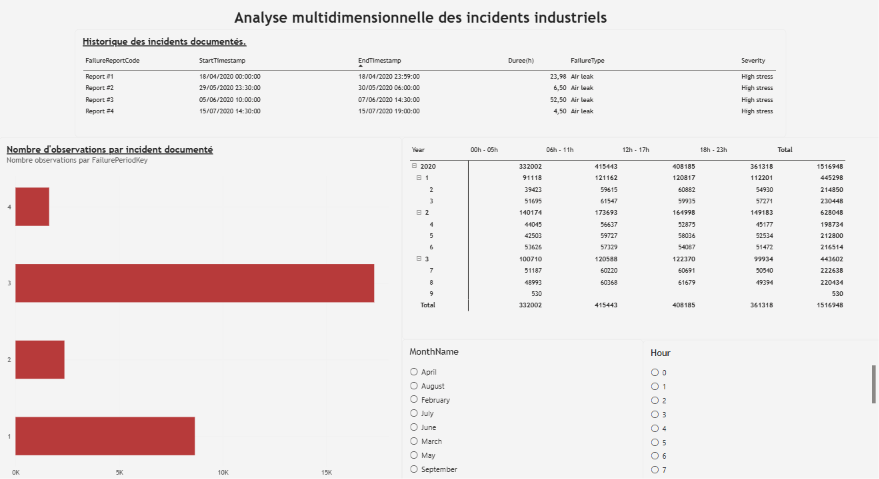
\includegraphics[width=\textwidth]{dashboard_3_incidents_olap.png}
\caption{Page Power BI Incidents et OLAP}
\label{fig:dashboard3}
\sourcefigure{capture réelle présente dans reports/figures}
\end{figure}
La page contient un historique tabulaire des quatre rapports, un histogramme du nombre d'observations par identifiant incident, une matrice temporelle et des segments MonthName et Hour. La table affiche Air leak et High stress pour les quatre lignes. Les durées visibles sont 23,98 h, 6,50 h, 52,50 h et 4,50 h, cohérentes avec les différences des bornes documentées.

La matrice présente Year en lignes et des tranches horaires en colonnes, avec un total général de 1\,516\,948. Cette structure illustre le pivot et le dice. Un utilisateur peut sélectionner un mois et une heure, puis observer le sous-ensemble correspondant. Le drill-down repose sur les niveaux de calendrier et doit conserver le contexte de filtre.

\section{Lecture OLAP}
Les trois pages couvrent les opérations suivantes :
\begin{itemize}
\item roll-up : passer des observations quotidiennes aux agrégats mensuels ;
\item drill-down : passer de Year à MonthName puis à CalendarDate ;
\item slice : sélectionner un seul FailureReportCode ;
\item dice : combiner un rapport avec MonthName et Hour ;
\item pivot : lire les heures en colonnes et les mois en lignes.
\end{itemize}
Power BI documente le drill comme une navigation dans une hiérarchie \cite{powerbiDrill}. Le projet doit cependant distinguer exploration OLAP et diagnostic : la visualisation organise les faits disponibles, elle ne remplace pas une expertise de maintenance.
